\documentclass{article}

\usepackage{amsmath}
\usepackage[margin=1cm]{geometry}
\usepackage{graphicx}
\usepackage{hyperref}
\usepackage{listings}

\title{
    \textbf{Programming Club}\\
    Fractals
}
\author{Hugh Leather}
\date{10$^{th}$ March 2015}

\begin{document}
    \maketitle
    
    \section{Pretty pictures}
        First let's have an easy way to make an image.  

        The simplest picture format you might use is PPM.  You can write out the image to a file in this format and then view it on your 
        desktop.
        
        You can, however use any way to show the image you like -- if your language lets you do graphical interfaces, then try that.
        
        The PPM format is:
        \begin{itemize}
            \item A ``magic number'' for identifying the file type. A ppm image's magic number is the two characters ``P3''.
            \item Whitespace (blanks, TABs, CRs, LFs).
            \item A width, formatted as ASCII characters in decimal.
            \item Whitespace.
            \item A height, again in ASCII decimal.
            \item Whitespace.
            \item The maximum colour value (Maxval), again in ASCII decimal. Must be less than 65536 and more than zero. Use 255 for 8 bit.
            \item A single whitespace character (usually a newline).
            \item A raster of Height rows, in order from top to bottom. Each row consists of Width pixels, in order from left to right.
            Each pixel is a triplet of red, green, and blue samples, in that order. Each sample is represented in pure binary by either 1
            or 2 bytes. If the Maxval is less than 256, it is 1 byte. Otherwise, it is 2 bytes. The most significant byte is first.
	    \item The pixel values are written in ASCII if the magic number is P3 and in binary if is P6.
            \item A row of an image is horizontal. A column is vertical. The pixels in the image are square and contiguous.
        \end{itemize}

	The following example shows the content of a ppm image with 5x5 white pixels.

	\begin{lstlisting}
		P3
		5 5
		255
		255 255 255  255 255 255  255 255 255  255 255 255  255 255 255
		255 255 255  255 255 255  255 255 255  255 255 255  255 255 255
		255 255 255  255 255 255  255 255 255  255 255 255  255 255 255
		255 255 255  255 255 255  255 255 255  255 255 255  255 255 255
		255 255 255  255 255 255  255 255 255  255 255 255  255 255 255      
	\end{lstlisting}

        If you can't see a PPM file on your system, try converting it with Image Magick:
        \begin{centering}
            \texttt{convert image.ppm image.jpg}
        \end{centering}
        
        \subsection{An Image Abstraction}
            Make a class (or other abstraction depending on your language) that encapsulates an RGB colour.
        
            Make a class (or other abstraction depending on your language) that encapsulates a simple image with a given width and height 
            and assumes 8 bit RGB.
            
            Give your class operations to set and get a pixel.
            
            Give your class an operation to write it to a file.

            Test your class by making an image that is 200x100 pixels, all red and writing to a file. 

            Test your class by making an image that is 200x100 pixels, with black at the top left pixel, red at the top right pixel,
            blue at the bottom left pixel, magenta at the bottom right, and smoothly interpolating in between.
    
            \begin{center}
                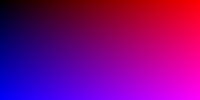
\includegraphics[width=0.4\textwidth]{smooth}
            \end{center}
    
    \section{Mandelbrots}
        Build a simple Mandelbrot display in any language you like.
        
        The Mandelbrot set is those complex points, $c$, for which $f_c(z)=z^2+c$ does not diverge when iterated.
        
        We'll take a pretty simple case, using the escape time algorithm.  That is, for a given point, $c$, start with 
        
        $$z_0 = 0$$
        $$z_n = z_{n-1}^2 + c$$
        
        Now iterate and find out the first $n$ for which $|z_n| > 2$ or $n > 32$ (the latter bit stops you going on forever).  
        
        This gives you number, $n$, in the interval, $[0,32]$. You can convert this number into a colour, making 0 black, 32 white, and
        interpolating in between.
        
        Now imagine your image ranges over the complex space, with the x axis ranging from -2 to 1, and the y axis ranging from
        -1.5\emph{i} to 1.5\emph{i}. You can now plot the Mandelbrot set for this part of the space. It should look like this:
        
        \begin{center}
            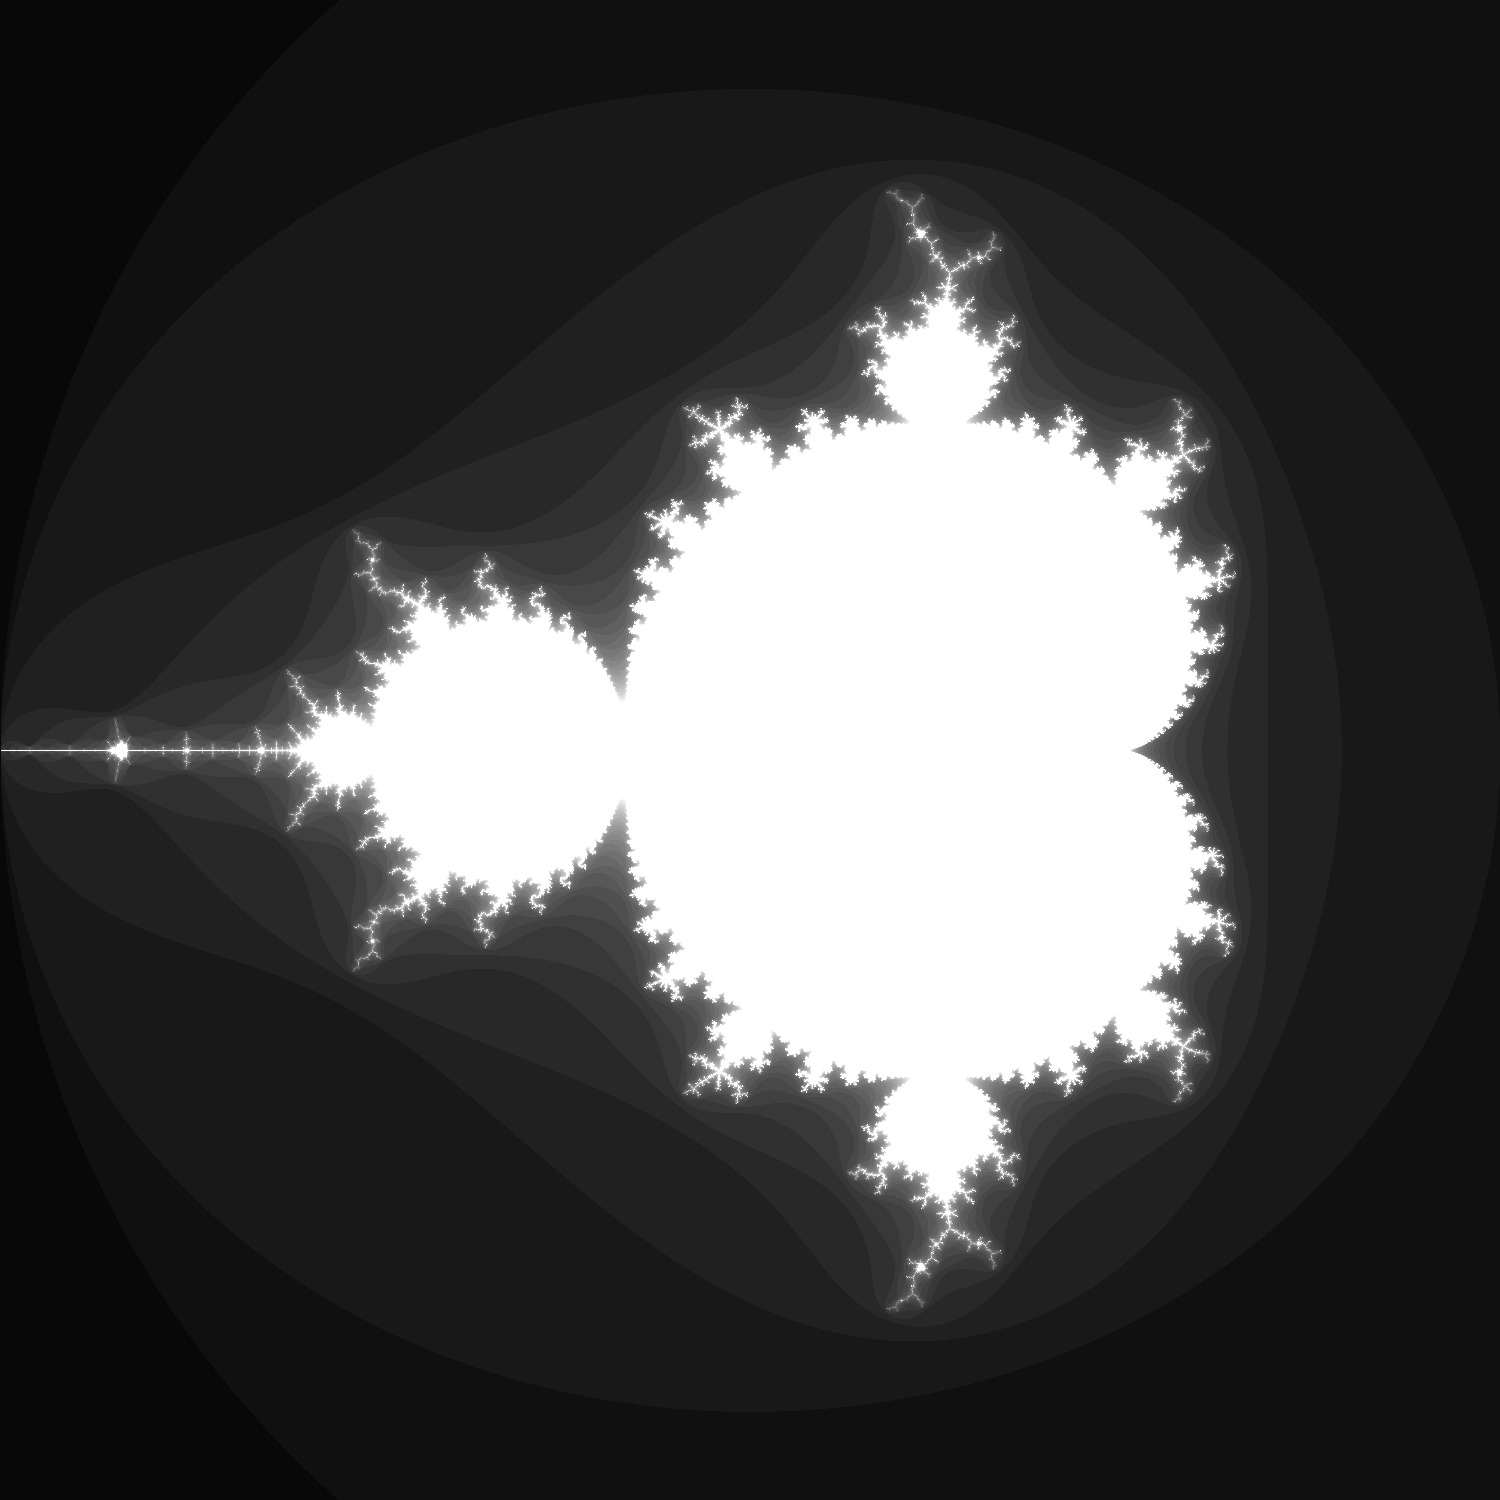
\includegraphics[width=0.4\textwidth]{mandelbrot}
        \end{center}
        
        Change the parameters and have a zoom about.
        
        \subsection{Other things}
            Here some ideas of things you might try (or move on to the next fractal).
            \begin{itemize}
                \item Build a GUI for it
                \item Try histogram colouring
                \item Try continuous colouring
                \item Do Multibrots - $z_n = z_{n-1}^d + c$, for some $d$
                \item Try contour or border mapping
                \item How do you go beyond 64 bit precision?
                \item Try showing Julia sets
            \end{itemize}
        \newpage
        
    \section{Brownian Trees}
        Here we're going to make very simple Brownian trees.  
        
        Choose a random x value and ``drop a flake of snow'' from the top of the image, straight down from the x axis, until there is a
        white pixel just below it, or one to left and below, or to the right and below, or until it hits the bottom. When it stops, leave
        it there in white. Repeat.
        
        Rather than dropping the snow a square at time, you can make it more efficient by remembering the highest value for each x
        coordinate and using that directly to work out where a bit of snow should stop.
        
        Finish when you can't drop snow more than one square.
        
        Do this on a 100x100 image, and you should get something that looks like this:
        
        \begin{center}
            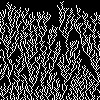
\includegraphics[width=0.4\textwidth]{snow}
        \end{center}
        

        You can make the colours more interesting by changing the colour to be near the colour you land on.        

    \section{Fractal Landscapes}
        Create a landscape with the diamond-square technique.  
        
        There is a very good explanation on Wikipedia, so I will just let you read that - 
        \url{https://en.wikipedia.org/wiki/Diamond-square_algorithm}
        
        Choose some good mapping for the heights to colours.  Here's one I did with sea, beach, forest, and snow capped mountains (note 
        this is with dimension $2^n$ using wrapping so it tiles with itself).
        
        \begin{center}
            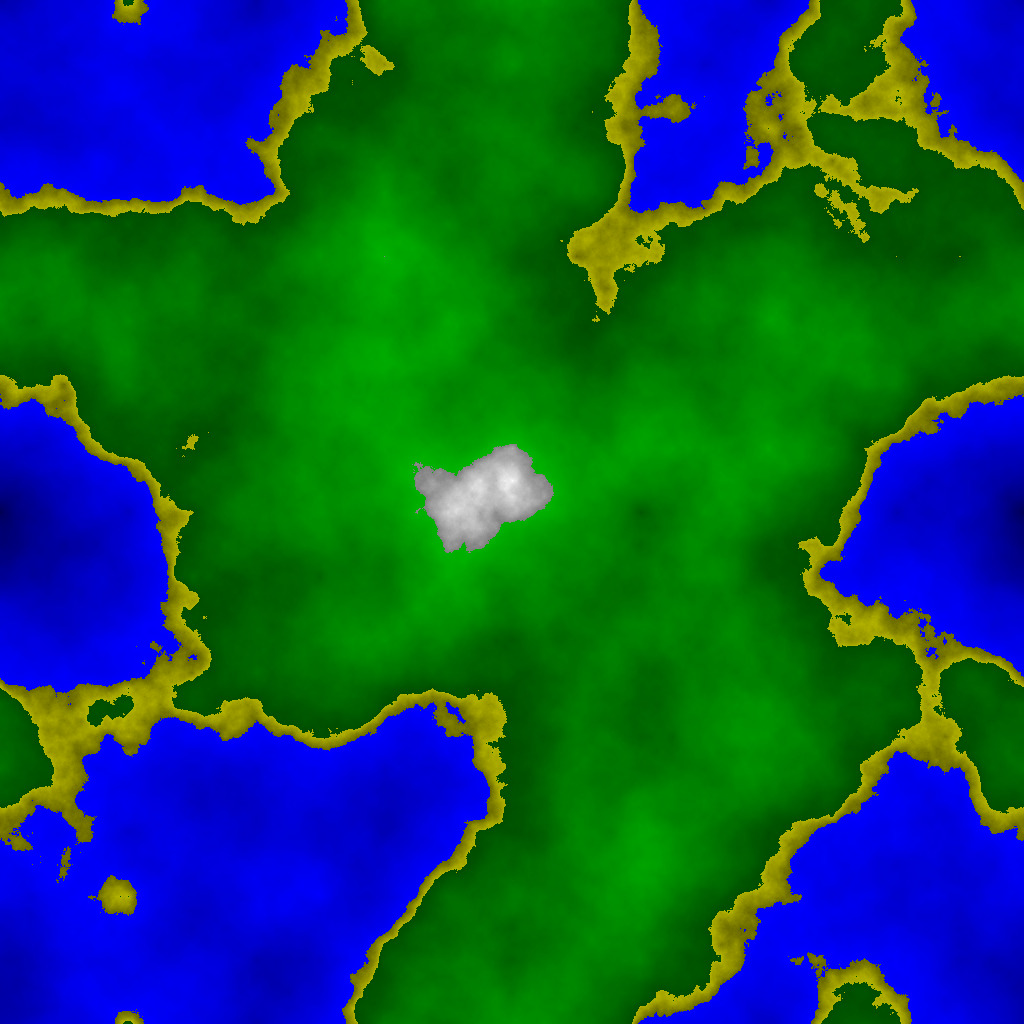
\includegraphics[width=0.4\textwidth]{land}
        \end{center}
        
        Find fast 3d package for your language and do a `fly over' of the landscape in the style of Zarch 
        \url{https://en.wikipedia.org/wiki/Zarch}.

\end{document}
